% Please do not change the document class
\documentclass{scrartcl}

% Please do not change these packages
\usepackage[hidelinks]{hyperref}
\usepackage[none]{hyphenat}
\usepackage{setspace}
\usepackage{graphicx}
\doublespace

% You may add additional packages here
\usepackage{amsmath}

% Please include a clear, concise, and descriptive title
\title{An Analysis of the Variability, Reliability, and Control Provided by Level Generation Techniques for 2D Platform Games}

% Please do not change the subtitle
\subtitle{COMP110 - Computer Architecture Essay}

% Please put your student number in the author field
\author{1507290}

\begin{document}

\maketitle

\abstract{There are a number of diverse approaches to level generation for 2D platform games, each placing emphasis on a different aspect of level generation. Chunk-based approaches tend to favour control and variation, whilst rhythm-based approaches favour playability and enjoyability. There are also evolutionary approaches that use genetic algorithms, which when combined with constraint satisfaction provide a high level of control and reliability. For an independent games developer with limited resources, generating creative, high quality levels with minimal human input is essential. This essay will present an analysis of the suitability of each approach.}

\section{Introduction}
Procedural content generation for 2D platform games is a relatively new field~\cite{compton:platform}. Many approaches to this problem have been developed, each with different characteristics~\cite{horn:comparative}. Chunk-based approaches, such as Occupancy-regulated Extension (ORE)~\cite{mawhorter:occupancy}, prioritise variability. Rhythm-based approaches, such as Launchpad~\cite{smith:launchpad}, place an emphasis on playability and enjoyment. Evolutionary approaches, such as Sorenson et al.'s~\cite{sorenson:generic}, provide a high level of control and reliability. For an independent games company who desire creative control yet do not possess the resources to hand design each level, the most desirable level generator would be one that requires minimal human input yet offers a high level of control. It should also generate interesting and playable levels consistently. 


%There are approaches which rely on hand-designed level chunks; methods that generate levels based on the rhythm of player actions; and evolutionary approaches that use genetic algorithms. For an independent games company who desire creative control yet do not possess the resources to hand design each level, the most desirable level generator would be one that requires minimal human input yet offers a high level of control whilst generating a wide variety of fun and playable levels consistently. 

\section{Comparison}

\subsection{Overview}
Smith et al.~\cite{smith:launchpad} base their level generation tool, Launchpad, on the concept of rhythm. They define rhythm as being an ideal sequence and timing of button presses; for example, a series of jumps. They use a two-tiered, grammar-based approach, as illustrated in Figure~\ref{fig:launchpad}, to ensure that rhythm is always present.
\begin{figure}[h]
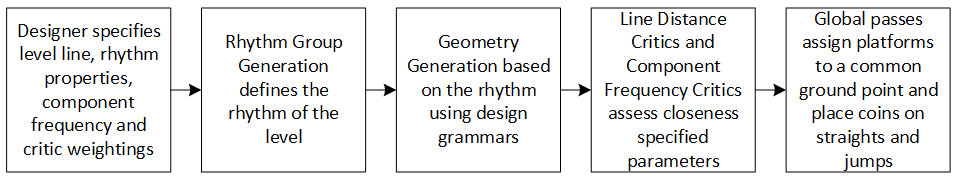
\includegraphics[width=\textwidth]{figs/launchpad.png}
\caption{Launchpad's Level Generation Process}
\label{fig:launchpad}
\end{figure}

Sorenson et al.~\cite{sorenson:generic} use a genetic algorithm combined with constraint satisfaction to generate levels, as illustrated in Figure~\ref{fig:genetic}. Their fitness function is inspired by rhythm, but unlike Launchpad, rhythm is defined as being alternating periods of high and low difficulty. Levels with a high fitness value are able to pass on their genetic information, resulting in levels gradually being improved. Constraint satisfaction is also used to ensure playability and provide additional control. 
\begin{figure}[h]
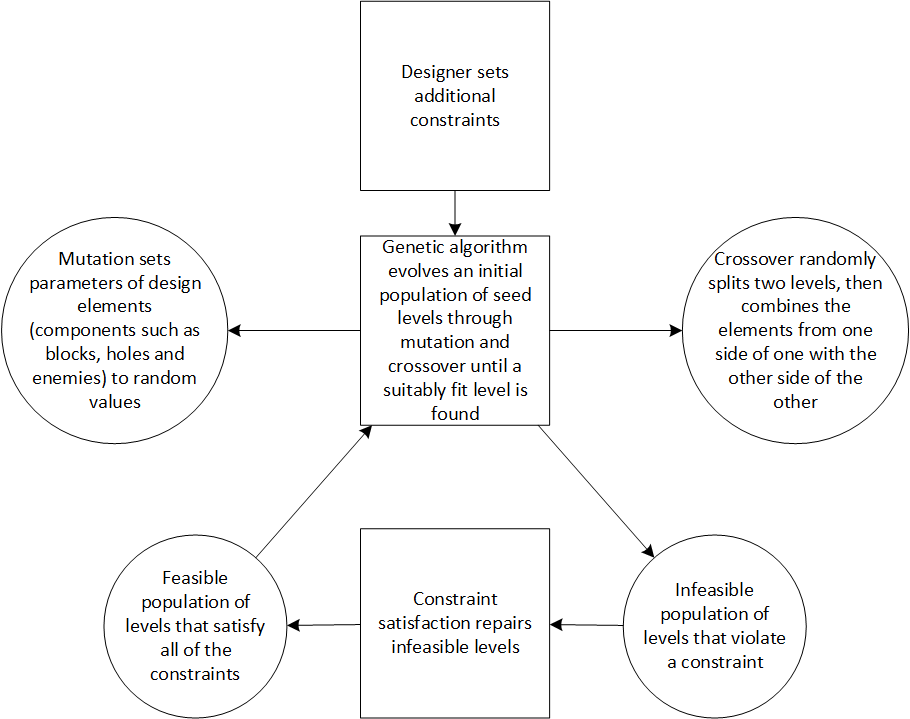
\includegraphics[width=\textwidth]{figs/genetic.png}
\caption{Sorenson et al.'s Level Generation Process}
\label{fig:genetic}
\end{figure}


Mawhorter and Mateas~\cite{mawhorter:occupancy} take a different approach to level generation. ORE uses pre-authored chunks of level and stitches them together based on anchor points that represent places the player can occupy, as illustrated in Figure~\ref{fig:ore}. Unlike the other two algorithms, ORE has no strict measures in place to ensure playability, as it was designed to prioritise variability.
\begin{figure}[h]
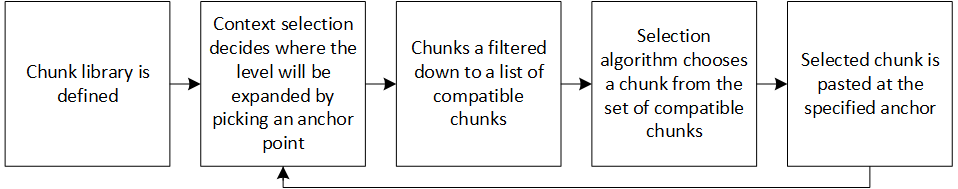
\includegraphics[width=\textwidth]{figs/ore.png}
\caption{Level Generation Process using Occupancy Regulated Extension}
\label{fig:ore}
\end{figure}


\subsection{Human Input and Control}
Launchpad~\cite{smith:launchpad} requires minimal effort whilst offering high levels of control. It allows the rhythm, the path of the level, and the frequency of each component to be specified. A large number of levels are generated before a pool of the best matches is presented. In practice, this means that Launchpad may be better for aiding the design of levels, rather than generating them in-game. Even if the closest matching level could automatically be chosen, generating a large pool of levels would extend the time taken.
 
Although other approaches using genetic algorithms have been developed~\cite{mourato:genetic}, Sorenson et al.'s~\cite{sorenson:generic} hybrid offers more direct control. In addition to allowing component numbers to be restricted, the difficulty of the generated levels can be adjusted by changing one parameter. Furthermore, levels can be generated around pre-authored level sections. This means that level profiles for each part of the game could be specified, allowing control over progression whilst maintaining variation. This could even allow levels to adapt to the player, by reducing the difficulty parameter if the player repeatedly loses\footnote{Although genetic algorithms are usually too slow to generate levels in-game, it is possible to find suitable levels quickly if the seed levels are well-designed~\cite{shaker:mario}.}.

Of the three methods, ORE~\cite{mawhorter:occupancy} requires the most human effort. Level chunks must be hand-authored, meaning that the output is greatly influenced by the quality of the chunks. Additionally, in order to achieve the desired result, an understanding of how the algorithm works is required.


\subsection{Flexibility and Variability}
Launchpad's~\cite{smith:launchpad} two-tiered approach allows levels with the same rhythm to have many geometric representations. The levels tend to be very linear and have little pattern variation~\cite{horn:comparative}, however, which could result in them lacking replayability. Additionally, the emphasis on rhythm means that the generated levels are only appropriate for dexterity-based platform games.

This is also the case with Sorenson et al.'s algorithm~\cite{sorenson:generic}, as the fitness function is modelled on challenge and difficulty with respect to skill. On the other hand, there is the scope to adjust the fitness function. If required, a fitness function based on a different model could be developed, allowing levels suitable for other types of platform games to be generated. Furthermore, their definition of rhythm is looser, allowing levels to be less linear and repetitive.

ORE~\cite{mawhorter:occupancy} could potentially generate levels appropriate for other types, such as exploration-based platform games with multiple paths. Chunks can be designed with any desired result in mind, whilst the algorithm does not need significant adjustment since the playability of levels is not assessed. Additionally, significant pattern variation and complex structures within generated levels can be observed~\cite{horn:comparative}, which could have a positive impact on the replayability of levels generated by ORE.


\subsection{Playability and Design} 
Launchpad~\cite{smith:launchpad} and Sorenson et al.'s~\cite{sorenson:generic} approach have measures in place to ensure playability. Launchpad has a physics engine that is aware of the movement speed and jump height of the player, which is used when generating the level geometry to ensure that the resulting level is possible to complete.
Sorenson et al. specify the playability requirements in the form of constraints, meaning that unplayable levels are repaired before being returned to the population of acceptable levels. 

ORE's~\cite{mawhorter:occupancy} focus on variability means that it has no measures in place to guarantee playability. This makes ORE unsuitable for generating levels in-game, as the player may be presented with an unbeatable level. An additional algorithm could be used to determine whether the level is playable before presenting it to the player, but that would use additional resources and extend the time taken.

Smith et al. and Sorenson et al. also ensure that some form of theoretical 'fun' is present in generated levels. Both of their definitions of fun are inspired by the concept of 'flow', as described by Csikszentmihalyi~\cite{csik:flow, smith:rhythm}. The fitness function used in Sorenson et al.'s algorithm is based on their comprehensive model of fun~\cite{sorenson:fun}, ensuring that the population evolves towards 'fun' levels. Smith et al. apply their definition of fun in the algorithm that generates the rhythm groups.

ORE is not based on any model of fun. This means that quality of the resulting level relies both on how well the chunks have been designed and the implementation of the chunk selection algorithm. With chunks designed by the authors of the algorithm, ORE came fourth in the \textit{2010 Mario AI Championship}~\cite{shaker:mario}, whilst Sorenson et al. managed to place third, despite their general approach.


\section{Conclusion}
Whilst ORE provides great control over the design of a generated level, Sorenson et al.'s approach and Launchpad provide greater flexibility and reliability with little effort. Sorenson et al.'s approach perhaps provides greater control than Launchpad. Parameters can easily be altered and level sections can be designed by hand if desired. The concept of 'fun' has been comprehensively modelled, ensuring that generated levels are enjoyable. This is demonstrated by their reasonable placing in the \textit{2010 Mario AI Championship}~\cite{shaker:mario}. Overall, Sorenson et al.'s approach would allow a small independent developer to reliably produce fun and playable levels with minimal effort, whilst providing a high level of creative control.


\bibliographystyle{ieeetran}
\bibliography{comp110_architecture}

\end{document}
